%%%%%%%%%%%%%%%%%%%%%Preâmbulo%%%%%%%%%%%%%%%%%%%%%%%%%%%%%%%%%%%%%%%%%%%%%

\documentclass[a4paper, 10pt]{article}
\usepackage[utf8]{inputenc}
\usepackage[left=3cm, top=3cm, right=2cm, bottom=2cm]{geometry}
\usepackage{setspace}
\setlength{\parindent}{1.25cm}
\usepackage{indentfirst}
\usepackage{graphicx}
\usepackage{caption}
\usepackage{babel}[portuguese]
\usepackage{float}
%%%%%%%%%%%%%%%%%%%Começo do Relatório%%%%%%%%%%%%%%%%%%%%%%%%%%%%%%%%%%%%%%%%%%%%%%%


\begin{document}
	\begin{center}
		
			\textbf{ 
\includegraphics[scale=0.06]{figs/ufpa.png}  \\UNIVERSIDADE  FEDERAL DO PARÁ \\ INSTITUTO DE CIÊNCIAS EXATAS E NATURAIS \\ FACULDADE DE ESTATÍSTICA}  
			
			\vspace{4cm}
	\end{center}
	
	\begin{center}
	    Jessica Teixeira Araujo
	\end{center}
    \\
    		\vspace{4cm}
        	\begin{center}	
        ANÁLISE DA QUALIDADE DE VIDA NO ESTADO DO PARÁ
		\end{center}
			
	\begin{center}
	\\
			
		\vspace{9cm}
			
			05 de Julho de 2022
			\\Belém-pa
	\end{center}
%%%%%%%%%%%%%%%%%%%%%%%%%%%%%%%%%%%%%%%%%%%%%%%%%%%%%%%%%%%%%%%%%%%%%%%%%%%%%%%%%%%%	
	\newpage
    \onehalfspacing 
       \begin{center}
         \Large
         \textbf{RESUMO}
       \end{center}
       \\
    O estudo avalia a qualidade de vida nos dez municípios do estado do Pará que apresentaram melhor IDHM no ano de 2010. Utilizando duas vertentes metodológicas: qualitativa e quantitativa. A primeira vertente baseou-se na Pirâmide de Maslow, para seleção das taxa e indicadores, que serão utilizados na segunda vertente. A segunda vertente, gerou perfis médios, e, elaborou-se um indicador composto capaz de classificar a qualidade de vida de forma mais atual que o IDHM empregado inicialmente. Dentre os resultados obtidos, houve confirmação na análise dos gráficos de pontos gerados pelos perfis médios e a classificação obtida atráves do indicador composto. E, por fim, concluiu-se que apesar do IDHM ser um indicador válido para os estudos relacionados a análise da qualidade de vida, o mesmo encontra-se ultrapassado. E, sugeriu-se que a periodicidade para a elaboração do IDHM não ultrapasse dois anos, visto que, a sociedade tem interesse em receber planejamento e medidas orçamentárias para a melhoria da qualidade de vida, não somente no estado do Pará, mas também a nível Brasil. 
    
    \\
    
    \noindent
    \textbf{Palavras-chave}: Qualidade de vida, IDHM, Pirâmide de Maslow, Indicador composto.
    
     \begin{center}
         \Large
         \textbf{ABSTRACT}
       \end{center}
   The study analyze the quality of life in the ten municipalities in the state of Pará that presented the best IDHM in 2010. Using two methodological approaches: qualitative and quantitative. The first strand was based on Maslow's Pyramid, for the selection of rates and indicators, which will be used in the second strand. The second aspect generated average profiles, and a composite indicator was elaborated capable of classifying quality of life in a more current way than the IDHM initially used. Among the results obtained, there was confirmation in the analysis of the graphs of points generated by the average profiles and the classification obtained through the composite indicator. Finally, it was concluded that although the IDHM is a valid indicator for studies related to the analysis of quality of life, it is outdated. And, it was suggested that the periodicity for the elaboration of the IDHM should not exceed two years, since society is interested in receiving planning and budgetary measures to improve the quality of life, not only in the state of Pará, but also at the Brazil.
    
    \noindent\textbf{Keywords}: Quality of life, IDHM, IQV, Maslow's Pyramide, Compound Indicator.
    
    \newpage
      \large
      \section{INTRODUÇÃO}
      \onehalfspacing 
    A análise da qualidade de vida é um tema muito complexo e difundido. Visto que, cada ser humano é único e possui necessidades conforme sua especifidade. Sendo assim, este estudo aborda os níveis teóricos, baseados na Pirâmide de Maslow, que um indivíduo necessita para alcançar a qualidade de vida tão almejada nos dias atuais.
    
    \\
    A seguir temos três citações sobre qualidade de vida, para refletirmos.
 
    \begin{quote}
    {“A percepção do indivíduo de sua inserção na vida, no contexto da cultura e sistemas de valores nos quais ele vive e em relação aos seus objetivos, expectativas, padrões e preocupações” Organização Mundial da Saúde (OMS).}
    \end{quote}
    
     \\
   
    \begin{quote}
    {“Qualidade de vida não é poder ganhar dinheiro e morar em condomínios fechados. Qualidade de vida é você caminhar à noite em sua cidade sem medo de ser assaltado.” Felipe Sandrin.}
    \end{quote}
    
    \\
    
     \begin{quote}
    {“Vivemos em um país de velhos com qualidade de vida! "Qualidade" aqui é um eufemismo que sofreu o mesmo desgaste da palavra "especial" para facilitar a inclusão social. Velho é velho e tem tudo geriátrico!” Claudeci Ferreira de Andrade.}
    \end{quote}
    
    \\
    Realizando-se uma simples busca no site acadêmico www.scielo.org, acessado no dia 02/07/2022 às 8:54 horas, utilizando-se a palavra "qualidade de vida" retornou a quantidade de 10.415 resultados dentre artigos, livros, monografias e entre outros. Logo, percebe-se que o termo é bastante difundido e que não existe uma definição que deve ser seguida como ouro.
    
    \\
    Portanto, em geral, a qualidade de vida envolve o bem estar espiritual, físico, mental, psicológico e emocional, além de relacionamentos sociais, como família e amigos e, também, saúde,  educação, habitação, saneamento básico e outras circunstâncias da vida.
    
    \\
    Uma das formas mais tradicionais de se avaliar qualidade de vida em grandes populações, no âmbito quantitativo, é o Índice de Desenvolvimento Humano (IDH). E que, segundo MINAYO, HARTS e BUSS (2000) tem por objetivo ser um indicador sintético de qualidade de vida.
    
    \\
    A seguir, temos o mapa geográfico com a faixa do IDHM no Brasil.
      
    \begin{figure}[H]
	\centering 
	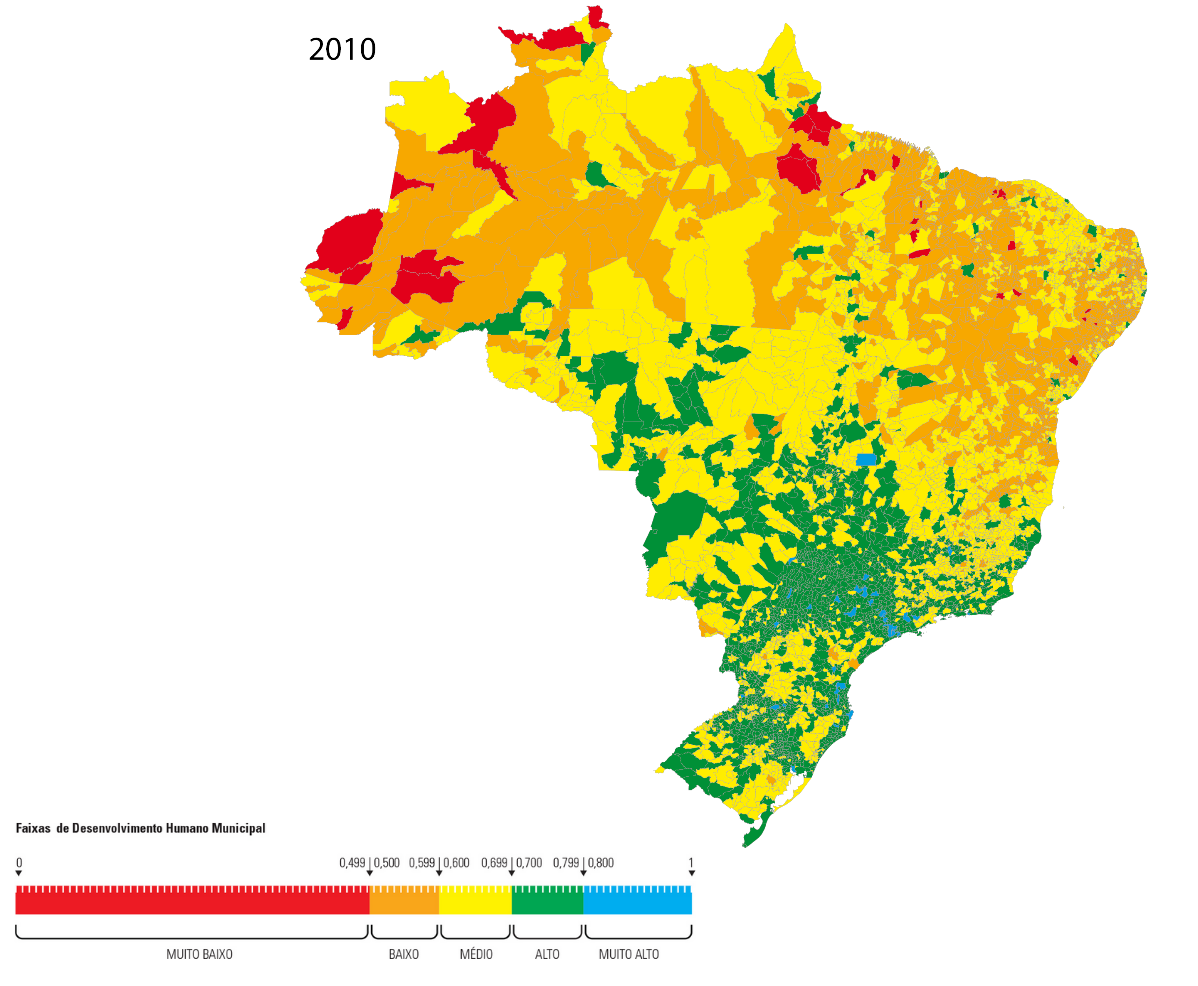
\includegraphics[scale=0.5]{figs/MAPA BRASIL IDHM 2010.png}
	\caption{\centering Mapa geográfico da faixa de IDHM no Brasil. \\ Fonte: Atlas Brasil, http://www.atlasbrasil.org.br/acervo/biblioteca.}
	\label{Fonte: Atlas Brasil, http://www.atlasbrasil.org.br/acervo/biblioteca}
	\end{figure}
\\
Observando o mapa acima verifica-se que o estado do Pará, em sua na maior parte, apresenta IDHM com classificação: muito baixo, baixo e médio. Sendo poucas as áreas que possuiem classificação alta e nenhuma classificada como muito alta.

\\

O estado do Pará possui 144 municípios que são distribuídos entre as 12º regiões de integração do estado. E, está situado na Região Norte, sendo o segundo maior estado do país em extensão territorial, com uma área de 1 245 870,798 km², também é classificado como a 13º maior subdivisão mundial.

\\

A população paraense estimada em 2021 foi de 8.777.124 habitantes e representa 4,11\% da população brasileira estimada em 2021. 

    \newpage
     
       \large
       \section{OBJETIVO}
    O estudo tem como objetivo avaliar a qualidade de vida da população paraense nos 10 municípios  que apresentam melhor índice de IDHM no estado. Em duas vertentes quantitativa e qualitativa.
       \onehalfspacing 
       
        \section{METODOLOGIA}
    
    A metodologia partiu da aplicação de duas vertentes no estudo, sendo elas: qualitati-va e quantitativa. Como ferramenta de análise qualitativa empregou-se a Pirâmide de Maslow. E, paralelamente, a análise quantitativa baseou-se no estudo das taxas e índices que possuem relação entre o IDHM e a Pirâmide de Maslow.
         
    \\
    Com a finalidade de refinar o objeto de estudo, dentre os 144 muincípios do Estado do Pará, classificou-se o IDHM do maior para o menor valor obtido. De acordo, com os dados fornecidos pelo PNUD (Programa das Nações Unidas para o Desenvolvimento Humano), órgão responsável pela a avaliação do IDHM, no último censo realizado em 2010.
    
    \\
    Os dez municípios alvo deste estudo serão: Belém, Ananindeua, Parauapebas, Santarém, Marituba, Novo Progresso, Castanhal, Canaã dos Carajás, Redenção e Marabá. A seleção, conforme classificação do IDHM, está representada na tabela a seguir:
    \\
        \begin{table}[H]
    \centering
	     \caption{\centering Municípios paraenses que apresentaram melhor IDHM em 2010.}
    \scalebox{1}{\begin{tabular}{c|c|c} \hline
	
	   Município & Posição IDHM & IDHM\\ \hline
		Belém & 79 & 0,746 \\ \hline
		Ananindeua & 107 & 0,718 \\ \hline
		Parauapebas & 110 & 0,715 \\ \hline
		Santarém & 134 & 0,691 \\ \hline
		Marituba & 149 & 0,676 \\ \hline
		Novo Progresso & 152 & 0,673 \\ \hline
		Castanhal & 152 & 0,673 \\ \hline
		Canaã dos Carajás & 152 & 0,673 \\ \hline
		Redenção & 153 & 0,672 \\ \hline
		Marabá & 157 & 0,668 \\ \hline
        	
        \end{tabular}} 
	\\ 
	Fonte: www.br.undp.org/content/brazil/pt/home/idh0/rankings/idhm-municipios-2010.html
	
	   \label{tab:my_label}
	\end{table} 
	
	\\
    \subsection{Pirâmide de Maslow}
     
     A Pirâmide de Maslow, também chamada de Teoria da Hierarquia das Necessidades Humanas, foi criada pelo psicólogo humanista norte-americano Abraham Maslow. Sua teoria foi ilustrada, pela primeira vez, na obra Teoria da Motivação Humana, de 1954. E, ela representa as necessidades humanas, das mais básicas às mais complexas. Sendo que, as pessoas possuem conjuntos de necessidades diferentes que se impõem umas sobre as outras, todas elas passíveis de classificação.
     
    \\
    Maslow expõe os fatores de satisfação do ser humano em cinco níveis, dispostos hierarquicamente, cada um formando um grupo de necessidades determinantes para que as pessoas atinjam suas satisfações pessoais e profissionais.
     
     \\
     
     O fato da teoria ter uma representação de uma pirâmide, demonstra que deve-se seguir os níveis para progressão, da base até o topo.

    \begin{figure}[1h]
	\centering 
	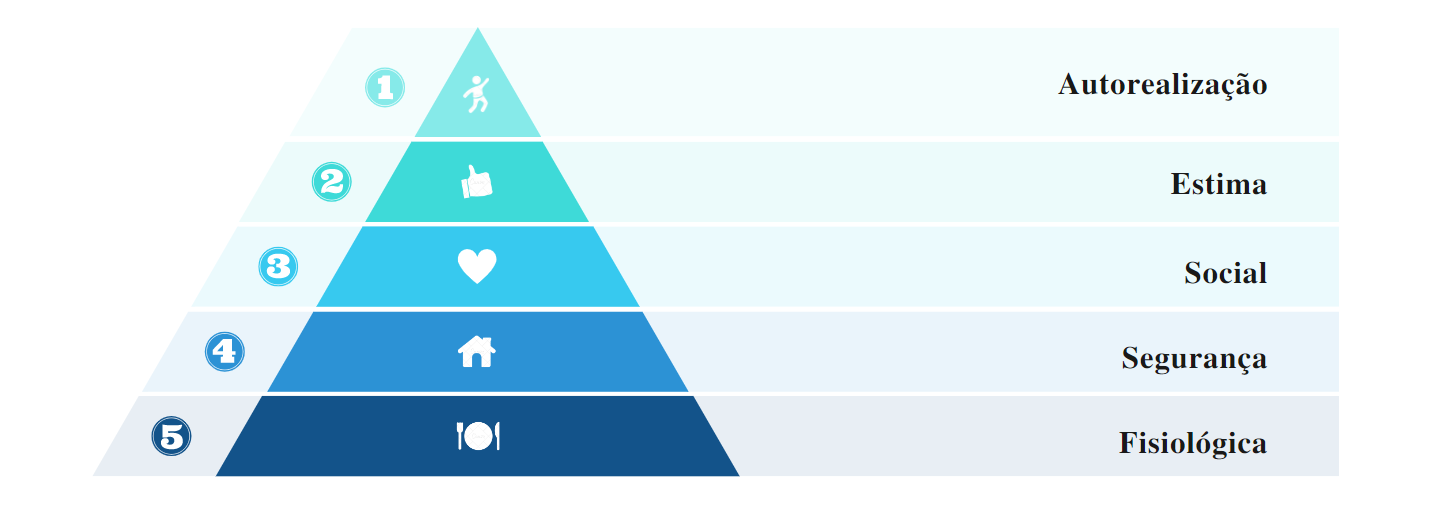
\includegraphics[scale=0.41]{figs/Maslow.png}
	\caption{Pirâmide de Maslow.\\Fonte: Elaboração própria.}
	\label{Fonte: Elaboração própria}
	\end{figure}
	
	\\
	
	As escalas da pirâmide de Maslow são representadas de maneira didática e funcional. As necessidades são detalhadas da base até o topo, como  explicado a seguir:
	\\
 - Fisiológicas: são as prioridades, as necessidades do organismo humano, como respiração, comida, água, sexo, sono, homeostase, excreção, etc.
 \\
- Segurança: são as estabilidades básicas, como segurança, saúde, segurança da família, segurança física em casos de violência. Ou seja, tudo vinculado à autopreservação.
\\
- Sociais: relação direta com nossos vínculos sociais, amizades, família, amor e demais ambientes de sociabilidade e pertencimento.
\\
- Estima: para se sentir competente e respeitada, a pessoa precisa receber retornos positivos e incentivos, desenvolvendo sua estima e sendo valorizada, seja no ambiente pessoal ou profissional. Como, por exemplo, confiança, conquista, respeito, reconhecimento, etc.
\\
- Autorrealização: nível focado em superação de desafios. Desenvolver autonomia decisória, ter flexibilidade, atuar com aquilo que deseja etc. 

\\
As necessidades de autorrealização são impossíveis de serem satisfeitas coletivamente, posto que não se trata de necessidades de um único indivíduo. Por sua vez, as necessidades fisiológicas são as mais simples de serem satisfeitas coletivamente, pois são necessidades básicas inerentes ao ser humano desde que nasce.

\\
Conclui-se que, conforme é conquistado variados componentes de uma mesma necessidade, a pessoa automaticamente sente-se mais apta para atingir as próximas etapas. E, quando uma necessidade não consegue ser satisfeita, às vezes gera frustrações e compor-tamentos negativos. E, sendo a teoria amplamente empregada na psicologia, gestão do conhecimento e recursos humanos.

\subsection{IDHM}

O Índice de Desenvolvimento Humano Municipal (IDHM) é uma unidade de medida utilizada para aferir o grau de desenvolvimento de uma determinada sociedade nos quesitos de educação, saúde e renda. A utilização de um indicador que envolvesse outras variáveis que não somente a questão econômica ocorreu pela primeira vez em 1990 pelo Programa das Nações Unidas para o Desenvolvimento (PNUD). 

\\
Esse indicador foi criado pelo paquistanês Mahbub Ul Haq e pelo indiano Amartya Sem. E, matematicamente, o índice representa uma média geométrica composta de  três IDHM's, e varia de 0 a 1. Quanto mais próximo de 1, maior o desenvolvimento humano daquele município. O IDHM ajusta o IDH para a realidade dos municípios e reflete as especificida-des e desafios regionais no alcance do desenvolvimento humano no Brasil.

\\
As três dimensões utilizadas no  IDHM, são: 
\\
- IDHM Longevidade: representa a oportunidade de viver uma vida longa e saudável. Por sua vez, é medida pela expectativa de vida ao nascer, calculada por método indireto a partir dos dados dos censos demográficos do IBGE. Esse indicador mostra o número médio de anos que as pessoas viveriam a partir do nascimento, mantidos os mesmos padrões de mortalida-de observados no ano de referência.
\\
-  IDHM Educação: representa a oportunidade de ter acesso ao conheci-mento. Leva-se em consideração o nível de conhecimento da população, ou seja, o grau de instrução. Sendo analisadas as taxas de alfabetização e a escolarização (educação infantil, educação fundamental, ensino médio e superior), que indicam a média de anos escolares de um adulto (a partir de 25 anos), bem como a média esperada para uma criança em idade escolar. São analisadas as taxas de evasão escolar, repetência e o oferecimento de vagas para as crianças aptas a serem matriculadas.
\\
- IDHM Renda: representa a oportunidade de ter um padrão de vida que garanta as necessidades básicas, representadas pela saúde, educação e renda. O padrão de vida é medido pela renda municipal per capita, ou seja, a renda média de cada residente de determinado município. Sendo, a soma da renda de todos os residentes, dividida pelo número de pessoas que moram no município - inclusive crianças e pessoas sem registro de renda. Os dados são do Censo Demográfico do IBGE.
	
A tabela à seguir, estão representados os dados dos IDHM's, referente aos municípios em estudo.
   
  \subsection{Taxas e indicadores relacionados ao IDHM e Pirâmide de Maslow}
    
    A seguir, será analisado os dados mais recentes de índices que possuem relevância relacionada ao IDHM e a Pirâmide de Maslow, dos municípios abordados neste estudo.
    
    \subsubsection{Segurança}
    
    Será utilizada duas taxas para medir a segurança, sendo elas:
    \\
    \noindent
    - Taxa de homicídios: é o índice que mede o número de homicídios por causas violentas ocorridos no município para cada 100 mil habitantes. São classificadas como letalidade violenta as seguintes ocorrências: homicídio doloso, lesão corporal seguida de morte, latrocínio e homicídio decorrente de oposição à intervenção policial. Sua periodicidade é anual, sendo que o órgão responsável é a Secretaria Municipal de Ordem Pública (SEOP).
    \\
	- Taxa do crime de roubo: é o índice que calcula os crimes contra o patrimônio com e sem emprego de violência e/ou ameaça. Considera o número de ocorrências criminais para cada 100 mil habitantes e inclui roubo (subtração de coisa alheia móvel com emprego de violência e/ou ameaça) e furto (subtração de coisa alheia móvel sem emprego de violência e/ou ameaça).
	
	\\
	Para interpretação dos dados, elaborou-se o perfil médio das taxas de homicídio e roubo. Sendo necessário, primeiramente remover a escala de 100.000 habitantes. E, para isto, bastou-se dividir o valor da taxa fornecida por 100.000, assim obtendo o valor da taxa de incidência anual na população total. Em seguida, foi feita a média artimética das taxas anuais, obtendo-se o perfil médio de cada município.
	
	 \subsubsection{População}
	  Será utilizada duas taxas para medir a população, sendo elas:
    \\
	  \noindent
	- População estimada: é uma projeção utilizando a tendência de crescimento, analisando-se os anos anteriores. As projeções e estimativas populacionais possue fundamental importância no cálculo de indicadores sociodemográficos nos períodos intercensitários, bem como alimentam as bases de informações de Ministérios e Secretarias Estaduais e Municipais da área social para a implementação de políticas públicas e posterior avaliação de seus respectivos programas. Além disso, em cumprimento ao dispositivo constitucional, as estimativas da população constituem o principal parâmetro para a distribuição, conduzi-da pelo Tribunal de Contas da União, das quotas relativas ao Fundo de Participação de Estados e Municípios.
    \\
    - Índice de Envelhecimento (IE): é uma forma de aferir quantitativa-mente o envelhecimento populacional. E, mede a relação entre a população idosa e a população jovem de 0 a 14 anos de idade. 
    
    \\
    Para interpretação dos dados, elaborou-se o perfil médio das taxas da população e IE. Atráves, de média artimética das taxas anuais, obtendo-se o perfil médio de cada município.
	
    \subsubsection{Renda}
     Será utilizada duas taxas para medir a renda, sendo elas:
     \\
     \noindent
	- Quantidade de vínculos empregatícios total no emprego formal: são a quantidade de empregos formais ativos, informados pelas empresas ao assinar a carteira de trabalho de um indivíduo.
	\\
	- Remuneração média do trabalhador formal: é o valor total da receita dos vínculos empregatícios formais dividido pela quantidade de vínculos empregatícios formais correspon-dente ao mesmo período.
	
	\\
	Para interpretação dos dados de vínculo empregatício total no emprego formal, criou-se a taxa da população formalmente empregada por município, sendo utilizada a quantidade de vínculos empregatício dividido pela estimativa populacional, em determinado ano no município. Em seguida, elaborou-se o perfil médio das taxas da população formalmente emprega-da e a renumeração média do trabalhador formal. Atráves, de média artimética das taxas anuais, obtendo-se o perfil médio de cada município.

    \subsubsection{Saúde}
     Será utilizada duas taxas para medir a saúde, sendo elas:
     \\
    \noindent
	- Taxa de natalidade: indica o número de nascidos vivos ao longo de um ano a cada mil habitantes. Nesse cálculo não é considerado o número de crianças que morreram após o nascimento ou que já nasceram mortas.
	\\
	- Taxa de mortalidade: indica o número de óbitos ao longo de um ano a cada mil habitantes.
	
\\
Para interpretação dos dados, elaborou-se o perfil médio das taxas de natalidade e mortalidade. Sendo necessário, primeiramente remover a escala de 1.000 habitantes. E, para isto, bastou-se dividir o valor da taxa fornecida por 1.000, assim obtendo o valor da taxa de incidência anual na população total. Em seguida, foi feita a média artimética das taxas anuais, obtendo-se o perfil médio de cada município.
	
	
 \subsubsection{Educação}
  O Índice de Desenvolvimento da Educação Básica (IDEB) funciona como um indicador nacional (0 a 10) que possibilita o monitoramento da qualidade da Educação pela população por meio de dados concretos, com o qual a sociedade pode se mobilizar em busca de melhorias. Foi criado em 2007, pelo Instituto Nacional de Estudos e Pesquisas Educacionais Anísio Teixeira (INEP), formulado para medir a qualidade do aprendizado nacional e estabelecer metas para a melhoria do ensino. O IDEB é calculado a partir de dois componentes: a taxa de rendimento escolar (aprovação) e as médias de desempenho nos exames aplicados pelo INEP. Os índices de aprovação são obtidos a partir do Censo Escolar, realizado anualmente. E, as médias de desempenho utilizadas são as da prova brasil, para escolas e municípios, e do Sistema de Avaliação da Educação Básica (SAEB), para os estados e o País, realizados a cada dois anos. 
  \\
  
  Será utilizada duas taxas para medir a educação, sendo elas:
  \\
 \noindent
 - IDEB dos anos iniciais: valor médio do IDEB obtido nas séries iniciais do ensino fundameltal, do 1º ano 5º ano.
 \\
 - IDEB dos anos finais: valor médio do IDEB obtido nas séries finais do ensino fundameltal, do 6º ano 9º ano.
 
 \\
Para interpretação dos dados, elaborou-se o perfil médio das taxas do IDEB anos iniciais e finais. Sendo necessário, primeiramente converter o valor obtido para taxa percentual. E, para isto, bastou-se multiplicar, o valor forncecido, por 100. Em seguida, foi feita a média artimética das taxas anuais, obtendo-se o perfil médio de cada município.
 
 \subsection{Indicador composto}
 \subsubsection{Conceito}
 Indicadores compostos, indicadores sintéticos ou índices sociais são elaborados pela aglutinação de dois ou mais indicadores simples, referentes a uma mesma ou diferentes dimensões da realidade social. São usados pela sua capacidade de síntese para avaliar um conceito abstrato, pois, permitem orientar de uma forma mais objetiva a priorização de recursos e ações de política social.
 
 \\
  \subsubsection{Metodologia aplicada para construção do indicador composto}

 Para a construção do indicador composto, foi utilizado o método de z-scores. E, representa quanto uma medida se afasta da média em termos de desvio padrão. Quanto maior a média z-core (Mz) melhor a situação medida pelo indicador composto.

 
 \\
 \newline
 \\
 Representado na fórmula à seguir:
 
 \\
 \begin{center}
 $Z=\frac{X-X{mím}}{X{máx}-X{mím}}$
 \end{center}
 \\
 Onde:
\\
\noindent
$X$: dado obtido do indicador no município;
\\
\noindent
$X{mín}$: dado mínimo obtido do indicador no conjunto de amostra (municípios);
\\
\noindent
$X{máx}$: dado máximo obtido do indicador no conjunto de amostra (municípios);

\\ 
E, para para  o z-score, o indicador composto é a média aritmética simples dos $z{_1}, z{_2}, z{_3}, z{_4}, z{_5}, z{_6}, z{_7}$ e $z{8}$. 
\\
\noindent
Onde:
\\
$z{_1}$: taxa de homicídio;
\\
$z{_2}$: taxa do crime de roubo;
\\
$z{_3}$: índice de envelhecimento;
\\
$z{_4}$: taxa da população formalmente empregada;
\\
$z{_5}$: taxa de natalidade;
\\
$z{_6}$: taxa de mortalidade;
\\
$z{_7}$: taxa do IDEB dos anos iniciais; e
\\
$z{_8}$: taxa do IDEB dos anos finais.
\\
\\

Os parâmetros (taxas e índices) escolhidos para a criação do indicador composto, são os citados acima. Sendo que, para o cálculo de $z$ foi utilizado somente o valor mais recentes de cada taxa ou índice. Ou seja, o dado apurado no útiltimo ano abservado de cada taxa ou índice. 

 \large
 \section{RESULTADO}
 
A partir dos perfis médios elaborados de cada taxa, gerou-se um gráfico de pontos. Eles representam de maneira mais intuitiva, o cenário que cada municipio apresenta em determinada taxa. E, possibilita a análise em relação aos municípios.

\\
Todos os perfis médios são dados em percentual. Com exceção da remuneração dada em reais.

\\
%%%%%%%%%%%%%%%%%%%Inserindo ggplots%%%%%%%%%%%%%%%%%%%%%%

 \begin{figure}[H]
	\centering 
	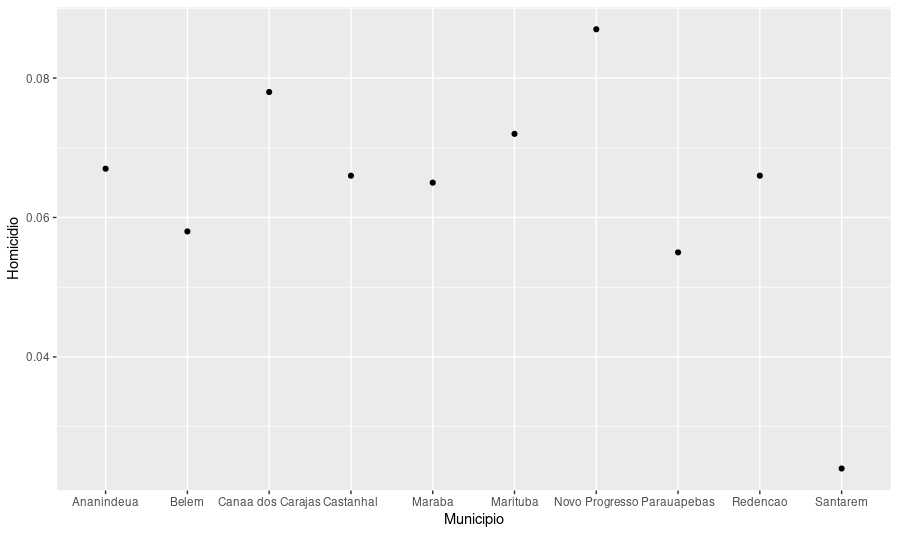
\includegraphics[scale=0.5]{HOMICIDIO.png}
	\caption{\centering Perfil médio da taxa de homicídio. \\ Fonte: Elaboração própria.}
	\label{}
	\end{figure}

%%%%%%%%%%%%%%%%%%%%%%%%%%%%%%%%%%%%%%%%%%%%%%%%%%%%%%%%%%%%%%%%%%%%%%%%%%%

    \begin{figure}[H]
	\centering 
	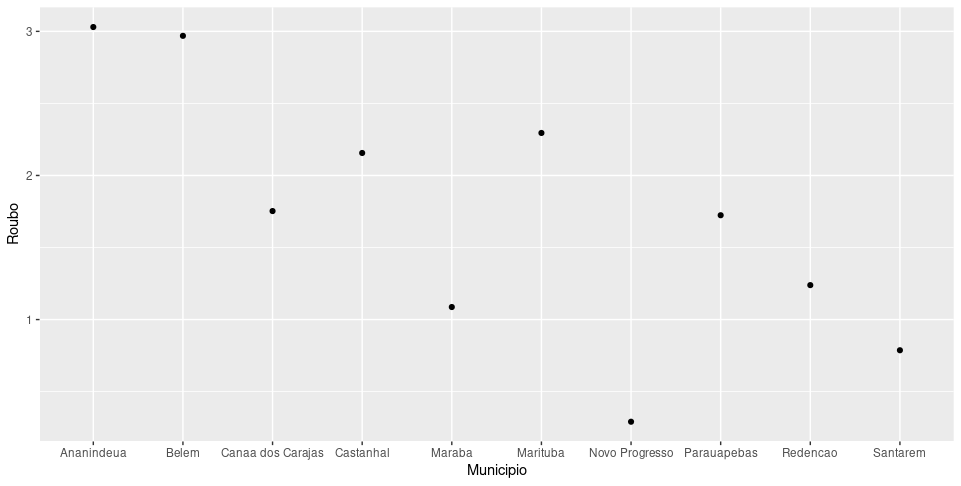
\includegraphics[scale=0.45]{ROUBO (1).png}
	\caption{\centering Perfil médio da taxa de crime de roubo. \\ Fonte: Elaboração própria.}
	\label{}
	\end{figure}
	
%%%%%%%%%%%%%%%%%%%%%%%%%%%%%%%%%%%%%%%%%%%%%%%%%%%%%%%%%%%%%%%%%%%%%%%%%%%
 \begin{figure}[H]
	\centering 
	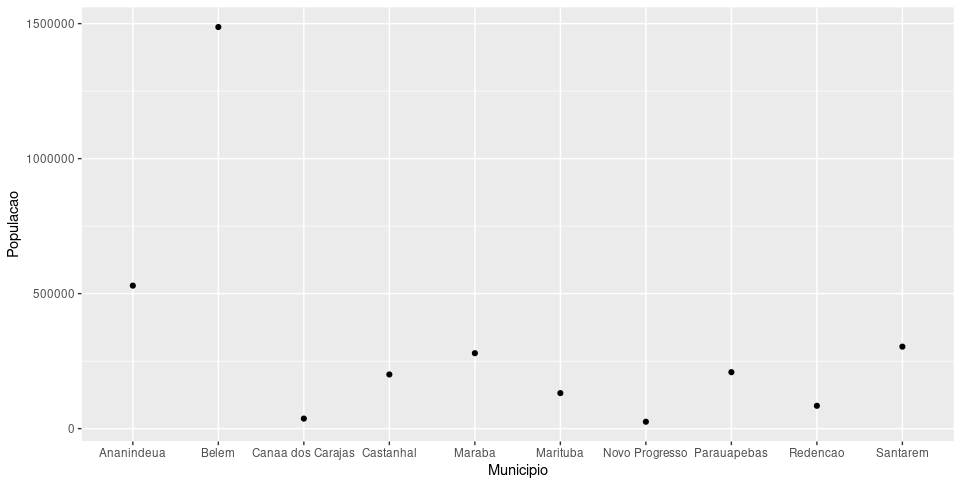
\includegraphics[scale=0.45]{POPULACAO.png}
	\caption{\centering Perfil médio da população. \\ Fonte: Elaboração própria.}
	\label{}
	\end{figure}
%%%%%%%%%%%%%%%%%%%%%%%%%%%%%%%%%%%%%%%%%%%%%%%%%%%%%%%%%%%%%%%%%%%%%%%%

 \begin{figure}[H]
	\centering 
	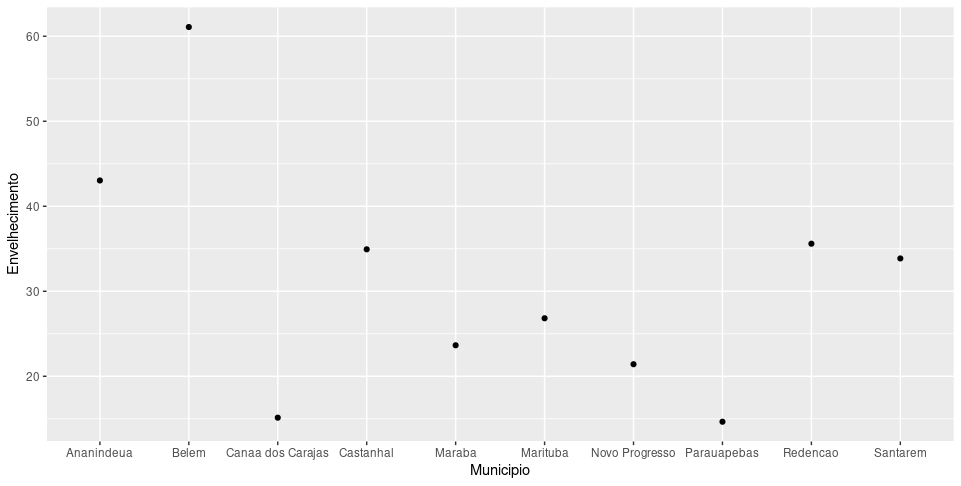
\includegraphics[scale=0.45]{ENVELHECIMENTO.png}
	\caption{\centering Perfil médio do índice de envelhecimento populacional. \\ Fonte: Elaboração própria.}
	\label{}
	\end{figure}
%%%%%%%%%%%%%%%%%%%%%%%%%%%%%%%%%%%%%%%%%%%%%%%%%%%%%%%%%%%%%%%%%%%%%%%%


 \begin{figure}[H]
	\centering 
	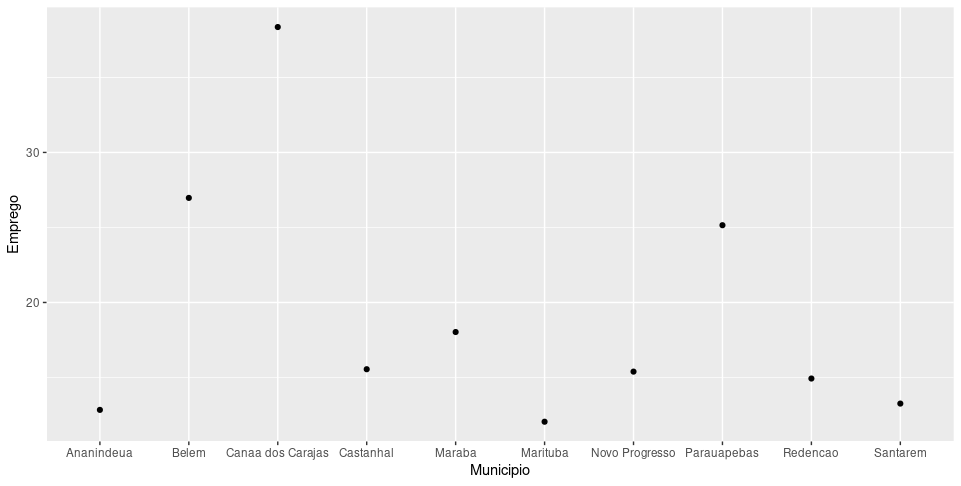
\includegraphics[scale=0.45]{EMPREGO.png}
	\caption{\centering Percentual da população formalmente empregada no ano de 2019. \\ Fonte: Elaboração própria.}
	\label{}
	\end{figure}
%%%%%%%%%%%%%%%%%%%%%%%%%%%%%%%%%%%%%%%%%%%%%%%%%%%%%%%%%%%%%%%%%%%%%%%%
%%%%%%%%%%%%%%%%%%%%%%%%%%%%%%%%%%%%%%%%%%%%%%%%%%%%%%%%%%%%%%%%%%%%%%%%


 \begin{figure}[H]
	\centering 
	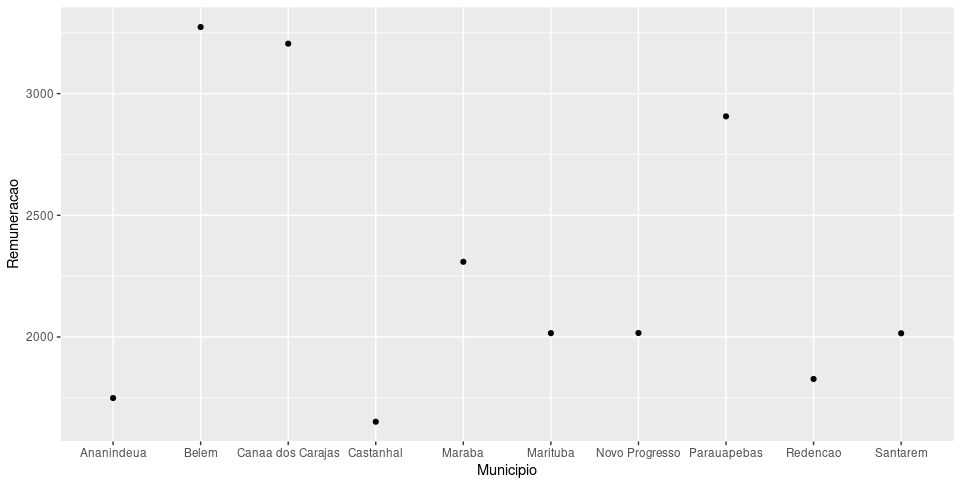
\includegraphics[scale=0.45]{REMUNERACAO.png}
	\caption{\centering Perfil médio da renumeração da população formalmente empregada. \\ Fonte: Elaboração própria.}
	\label{}
	\end{figure}
%%%%%%%%%%%%%%%%%%%%%%%%%%%%%%%%%%%%%%%%%%%%%%%%%%%%%%%%%%%%%%%%%%%%%%%%

 \begin{figure}[H]
	\centering 
	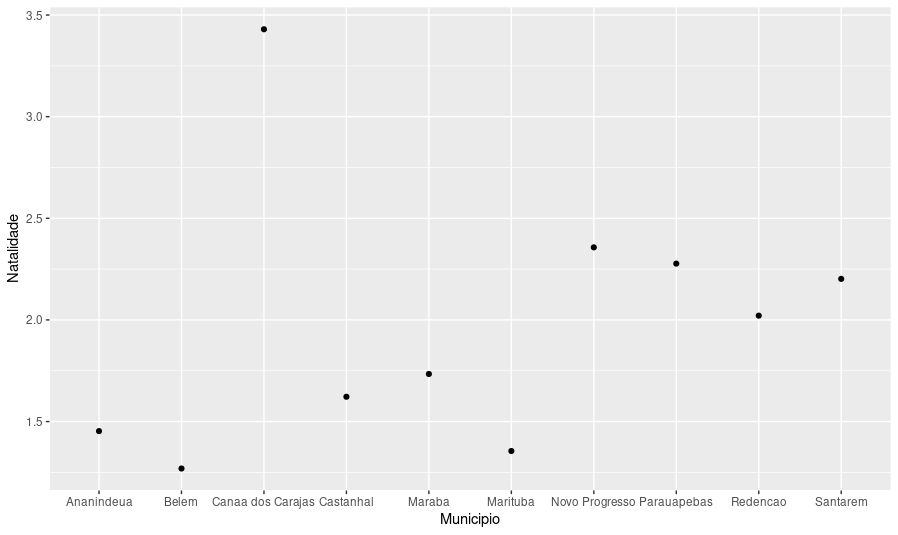
\includegraphics[scale=0.48]{NATALIDADE.png}
	\caption{\centering Perfil médio da taxa de natalidade na população. \\ Fonte: Elaboração própria.}
	\label{}
	\end{figure}
%%%%%%%%%%%%%%%%%%%%%%%%%%%%%%%%%%%%%%%%%%%%%%%%%%%%%%%%%%%%%%%%%%%%%%%%

 \begin{figure}[H]
	\centering 
	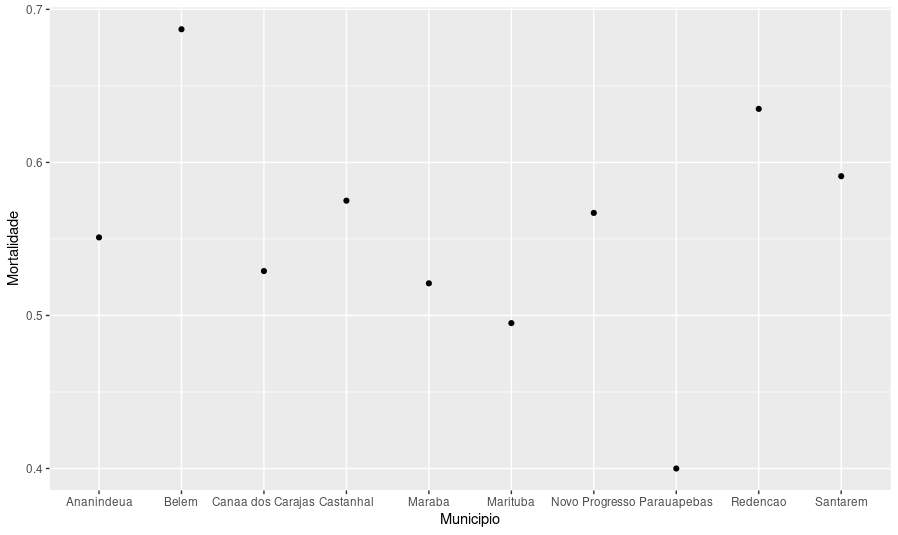
\includegraphics[scale=0.48]{MORTALIDADE.png}
	\caption{\centering Perfil médio da taxa de mortalidade na população. \\ Fonte: Elaboração própria.}
	\label{}
	\end{figure}

%%%%%%%%%%%%%%%%%%%%%%%%%%%%%%%%%%%%%%%%%%%%%%%%%%%%%%%%%%%%%%%%%%%%%%%%
\begin{figure}[H]
	\centering 
	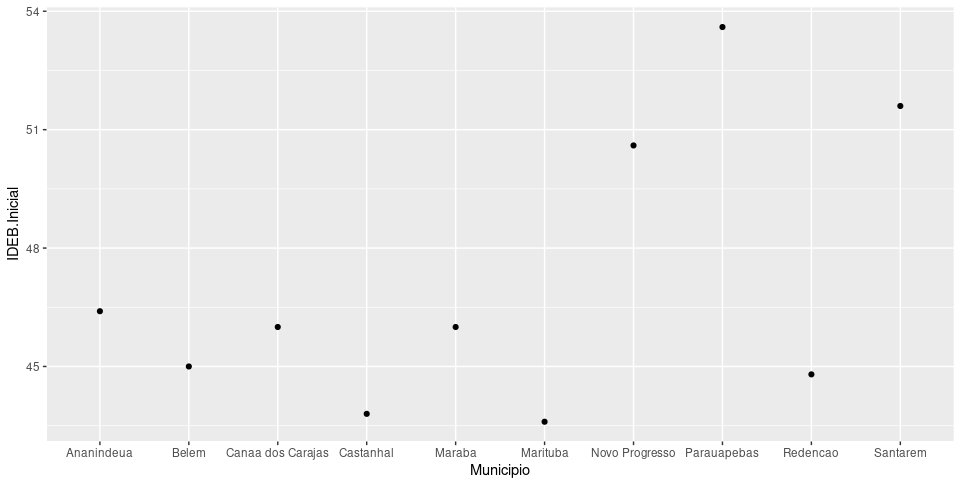
\includegraphics[scale=0.45]{IDEBINICIAL.png}
	\caption{\centering Perfil médio do IDEB dos anos iniciais. \\ Fonte: Elaboração própria.}
	\label{}
	\end{figure}
%%%%%%%%%%%%%%%%%%%%%%%%%%%%%%%%%%%%%%%%%%%%%%%%%%%%%%%%%%%%%%%%%%%%%%%%

\begin{figure}[H]
	\centering 
	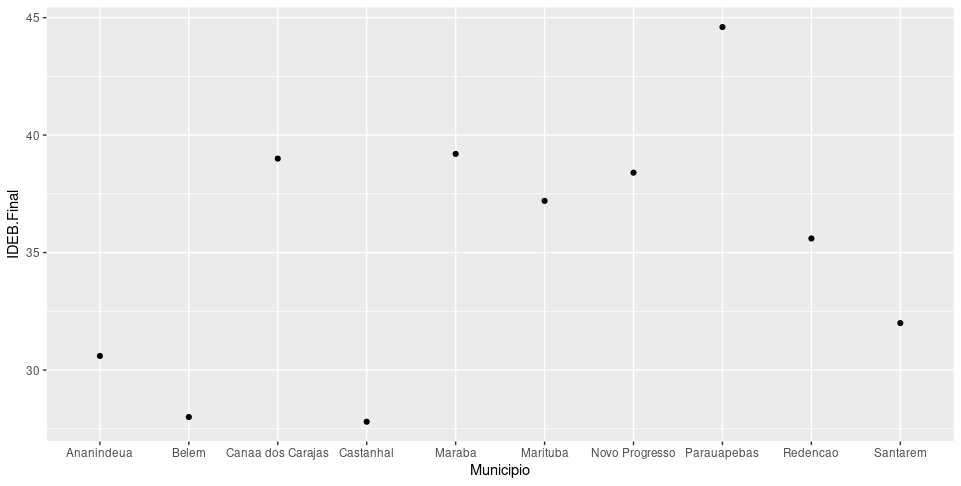
\includegraphics[scale=0.45]{IDEBFINAL.png}
	\caption{\centering Perfil médio da taxa de mortalidade na população. \\ Fonte: Elaboração própria.}
	\label{}
	\end{figure}
%%%%%%%%%%%%%%%%%%%%%%%%%%%%%%%%%%%%%%%%%%%%%%%%%%%%%%%%%%%%%%%%%%%%%%%%	
\\

A figura 3, sugere que durante os anos de 2016 a 2020 o município de Novo Progresso foi o que apresentou a maior taxa, proporcionalmente a sua população, e, o município de Santarém apresentou a menor taxa observada no mesmo período.

\\

A figrura 4, demonstra que durante os anos de 2016 a 2020 o município de Ananin-deua foi o que apresentou a maior taxa, seguido por Belém e Castanhal. E, o município de Novo Progresso apresentou a menor taxa observada no mesmo período.

\\

A figura 5, apresenta que durante o período de 2017 a 2021 o município de Belém mantem-se como o maior centro populacional. E, o município de Novo Progresso é o que apresenta menor população dentre os estudados.

\\

A figura 6, mostra que mais de 60\% da população Belenense poussui idade supeior a 14 anos de idade, enquanto, o município de Parauabepas apresenta, aproximadamente, apenas 15\%.

\\

A figura 7, mostra Canaã dos Carajás com o maior pencentual de população empregada formalmente em 2019, seguido por Belém e Parauabepas. Isso demonstra que nos grandes polos insutriais existe a maior oferta de empregos dormais. E, há dois casos que devem ser analisados isoladamente, o município de Ananindeua e Marituba, pois fazem parte da região metropolitana da capital paraense. E, é de conhecimento comum que por serem áreas de cornubação ligadas a capital, ocorre que habitantes das cidades proximas, como por exemplo Ananindeua e Marituba, viajem para trabalhar na capital diariamente.

\\

A figura 8, revela Belém, Canaã dos Carajás e Parauabepas com maior remuneração média durante os anos de 2015 a 2019. E, Castanhal possui o menor valor de remuneração média no mesmo período analisado. 

\\

A figura 9, o município de Canaã dos Carajás possui elevada taxa de natalidade no período de 2016 a 2020, enquanto Belém possui a menor taxa.

\\

A figura 10, observa-se Belém com elevada taxa de mortalidade no período de 2016 a 2020, enquanto Parauabepas possui a menor taxa.

\\

A figura 11, mostra que o município de Parauapebas apresentou melhor perfil médio no IDEB nos anos iniciais da educação pública, durante os anos de 2011 a 2019. E, o município de Marituba com menor rendimento.


\\

A figura 12, mostra que o município de Parauapebas apresentou melhor perfil médio no IDEB nos anos finais da educação pública, durante os anos de 2011 a 2019. E, o município de  Castanhal com menor rendimento.

\\

Diante da análise gráfica, e, buscando comparar o IDHM 2010 com os indicadores mais atuais elaborou-se um indicador composto por 8 parâmetros, citados na metodologia, que serão explicados melhor no decorrer da demosntração dos resultados do indicador.

\\
\begin{table}[H]
    \centering
	     \caption{\centering Dados utilizados para aplicação do metódo z-score.}
    \scalebox{1}{\begin{tabular}{c|c|c|c|c|c|c|c|c} \hline
	
Município & Hom. & Roub. & Env. & Emp.& Nat. & Mort. & ID.In & ID.Fi\\ \hline
Belém & 0.028\% & 1.715\% & 68.70\% & 26.968\% & 1.130\% & 0.867\% & 52.00\% & 41.00\% \\ \hline
Ananindeua & 0.026\% & 	1.836\% & 49.29\% & 12.840\% & 1.512\% & 0.698\% & 53.00\% & 43.00\% \\ \hline
Parauapebas & 0.047\% & 1.377\% & 15.98\% & 25.146\% & 1.285\% & 0.655\% & 56.00\% & 45.00\% \\ \hline
Santarém & 0.016\% & 0.534\% & 37.17\% & 13.263\% & 3.181\% & 	0.627\% & 55.00\% & 46.00\% \\ \hline
Marituba & 0.034\% & 1.138\% & 29.77\% & 12.046\% & 2.184\% & 	0.470\% & 49.00\% & 39.00\% \\ \hline
Novo Progresso & 0.093\% & 0.264\% & 23.75\% & 	15.395\% & 1.871\% & 0.725\% & 	56.00\% & 45.00\% \\ \hline
Castanhal & 0.037\% & 	1.604\% & 38.46\% & 15.549\% & 	1.239\% & 0.539\% & 48.00\% & 	37.00\% \\ \hline
Canaã dos Carajás & 0.073\% & 	0.879\% & 15.59\% & 38.361\% & 	1.611\% & 0.554\% & 51.00\% & 42.00\% \\ \hline
Redenção & 0.062\% & 0.827\% & 	40.30\% & 14.929\% & 2.383\% & 	0.629\% & 50.00\% & 40.00\%  \\ \hline
Marabá & 0.037\% & 0.736\% & 25.77\% & 	18.032\% & 2.119\% & 0.734\% & 	51.00\% & 43.00\%  \\ \hline
Máximo & 0.093\% & 1.836\% & 68.70\% & 	38.361\% & 3.181\% & 0.867\% & 	56.00\% & 46.00\%  \\ \hline
Mínimo & 0.016\% & 0.264\% & 15.59\% & 	12.046\% & 1.130\% & 0.470\% & 	48.00\% & 37.00\% \\ \hline
Média & 0.045\% & 1.091\% & 34.478\% & 	19.253\% & 1.852\% & 0.650\% & 	52.10\% & 42.10\% \\ \hline
Desvio Padrão & 0.024\% & 0.530\% & 16.192\% & 	8.414\% & 0.634\% & 0.114\% & 2.846\% & 2.885\% \\ \hline
        \end{tabular}} 
	\\ 
	Fonte: Elaboração própria.

	\\
	  \label{tab:my_label}
	\end{table} 

\begin{table}[H]
    \centering
	     \caption{\centering Dados obtidos utilizando o metódo z-score.}
    \scalebox{1}{\begin{tabular}{c|c|c|c|c|c|c|c|c} \hline
	
Município &$z{_1}$ & $z{_2}$ & $z{_3}$ & $z{_4}$ & $z{_5}$ & $z{_6}$ & $z{_7}$ & $z{_8}$ \\ \hline
Belém & -0.7398 & 1.1782 & 2.1135 & 0.917 & -1.1373 & 1.9049 & -0.0351 & -0.38131 \\ \hline
Ananindeua & 1.103 & 3.4653 & 3.0441 & 1.5261 & 2.3833 & 6.1217 & 18.6223 & 14.90558 \\ \hline
Parauapebas & 0.9812 & 1.5995 & -0.0131 & 1.9887 & 1.0255 & 4.7446 & 18.6764 & 14.59886 \\ \hline
Santarém &  0.6835 & 1.0089 & 2.2956 & 1.5764 & 5.0141 & 5.499 & 19.325 & 15.9455 \\ \hline
Marituba &  1.4415 & 2.1478 & 1.8386 & 1.4317 & 3.4426 & 4.1221 & 17.2168 & 13.51901 \\ \hline
Novo Progresso &  3.9022 & 0.4982 & 1.4668 & 1.8298 & 2.9492 & 6.3585 & 19.6764 & 15.59886 \\ \hline
Castanhal &  1.5459 & 3.0278 & 2.3753 & 1.8481 & 1.953 & 4.7272 & 16.8655 & 12.82573 \\ \hline
Canaã dos Carajás & 3.0786  & 1.6597 & 0.9628 & 4.5594 & 2.5394  & 4.8588 & 17.9196 & 14.55894  \\ \hline
Redenção & 2.595 & 1.562 & 2.4889 & 1.7744 & 3.7562 & 5.5166 & 17.5682 & 13.86565  \\ \hline
Marabá &  1.5514 & 1.3888 & 1.5916 & 2.1432 & 3.3401 & 6.4375 & 17.9196 & 14.90558 \\ \hline

        \end{tabular}} 
	\\ 
	Fonte: Elaboração própria.

	\\
	  \label{tab:my_label}
	\end{table}
\\
\noindent
Onde:
\\
$z{_1}$: z-score da taxa de homicídio;
\\
$z{_2}$:  z-score da taxa do crime de roubo;
\\
$z{_3}$:  z-score do índice de envelhecimento;
\\
$z{_4}$:  z-score da taxa da população formalmente empregada;
\\
$z{_5}$:  z-score da taxa de natalidade;
\\
$z{_6}$:  z-score da  taxa de mortalidade;
\\
$z{_7}$:  z-score da  taxa do IDEB dos anos iniciais; e
\\
$z{_8}$:  z-score da taxa do IDEB dos anos finais.

\begin{table}[H]
    \centering
	     \caption{\centering Classificação dos municípios de acordo com o indicador composto.}
    \scalebox{1}{\begin{tabular}{c|c} \hline

Município &  $M{_z}$ \\ \hline
Novo Progresso & 5.8089\\ \hline
Santarém & 5.7053\\ \hline
Ananindeua & 5.6857\\ \hline
Canaã dos Carajás & 5.5708\\ \hline
Marabá & 5.4753\\ \hline
Redenção & 5.4586\\ \hline
Castanhal & 5.8089\\ \hline
Marituba & 5.0178\\ \hline
Parauapebas & 4.8446\\ \hline
Belém & 0.4245\\ \hline

 \end{tabular}} 
	\\ 
	Fonte: Elaboração própria.

	\\
	  \label{tab:my_label}
	\end{table}
\\
\\
\noindent
Onde:
\\
 $M{_z}$: Média z-score = Indicador composto.

\\

Quanto maior a pontuação obtida em $M{_z}$ melhor é a situação medida pelo indicador composto. Sendo assim, a pontuação obtida confirma a análise dos perfis médios representa-dos nos gráficos. E, demonstra que atualmente o cenário dos IDHM's municipais, com relação ao censo de 2010, será alterado consideravelmente. 
\newpage
\large
\section{CONCLUSÃO}
\\
 Apartir da análise dos perfis médios e do indicador composto elaborado. Observou-se que não se pode utilizar os dados do IDHM do ano de 2010, visto que, o mesmo está ultrapassado e não reflete mais o cenário municipal.
 
 \\
 
 Sugiro, com este trabalho, que o IDHM seja medido com a periodicidade de no máximo dois anos. Visto que, cada município deveria inserir em suas políticas públicas e medidas orçamentárias, para o avanço da qualidade de vida municipal.  Pois, a sociedade possui interesse em receber planejamento e medidas orçamentárias para a melhoria da qualidade de vida, não somente no estado do Pará, mas também a nível Brasil. 
 
 \\
 
 Em termos de instrumentos de planejamento e orçamento o modelo brasileiro é definido na Constituição Federal de 1988 do Brasil, e, é composto por três instrumentos:  PPA (Plano Plurianal), LDO (Lei de Diretrizes Orçamentárias) e LOA (Lei Orçamentária Anual).
 
 \\
 
 O PPA possui vigência de quatro anos, e, tem como função estabelecer as diretrizes, objetivos e metas de médio prazo da administração pública. Cabe à LDO, anualmente, enunciar as políticas públicas e respectivas prioridades para o exercício seguinte. E, a LOA tem como principais objetivos estimar a receita e fixar a programação das despesas para o exercício financeiro.
 
 \\
 Assim, a LDO ao identificar no PPA as ações que receberão prioridade no exercício seguinte torna-se o elo entre o PPA, que funciona como um plano de médio-prazo do governo, e a LOA, que é o instrumento que viabiliza a execução do plano de trabalho do exercício a que se refere.
 
 \\
 %%%%%%%%%%%%%%%%%%%%%%%%%%%%%%%%%%%%%%%%%%%%%%%%%%%%%%%%%%%%%%%%%%%%%%%%%%%%%%%%%%%%%%%%%%%%%%%%%%%%%%%%%%%%%%%%%%
 COMENTAR SOBRE:  INSTRUMENTO DE PLANEJAMENTO E ORÇAMENTO.
\\
%%%%%%%%%%%%%%%%%%%%%%%%%%%%%%%%%%%%%%%%%%%%%%%%%%%%%%%%%%%%%%%%%%%%%%%%%%%%%%%%%%%%%%%%%%%%%%%%%%%%%%%%%%%%%%%%%%%%%%%%%%%%%%%%%%%%%%%%%%%%%%%%%%%%%%%%%%%%%%%%%%%%%%%%%%%%%%%%%%%%%%%%%%%%%%%%%%%%%%%%%%%%%%%%%%%%%%%%%%%%%%%%%%%%%%%%%%%%%%%%%%%%%%
\newpage
     
       \large
       \section{REFERÊNCIA BIBLIOGRAFICA}
\noindent 
AMARAL, Ernesto Friedrich de Lima. 2009. Elaboração de Indicadores Sociais. Aula PPT, UFMG.
\\
Cavassani, Amarildo Pereira; Cavassani, Edlene Barbieri; Biazin, Celestina Crocetta.
(2006). Qualidade de vida no trabalho: fatores que influenciam as organizações. XIII
SIMPEP – Bauru, SP, Brasil.
\\
Chiavenato, Idalberto. (1991). Recursos humanos na empresa. São Paulo: Atlas.
Chiavenato, Idalberto. (2006). Princípios da administração: o essencial em teoria
geral da administração. Rio de Janeiro: Editora Elsevier.
\\
Chiavenato, Idalberto. (1999). Gestão de pessoal: o novo papel dos recursos
humanos nas organizações. 13ª Ed. Rio de Janeiro: Campus.
\\
Ciconelli, Rozana Mesquita; Ferraz, Marcos Bosi; Santos, Wilton; Meinão, Ivone;
Quaresma. (1999, Maio/Junho), Marina Rodrigues. Tradução para a língua
portuguesa e validação do Questionário genérico de avaliação de qualidade de vida
SF-36 (Brasil SF-36). Revista Brasileira de Reumatologia – Vol. 39 – Nº 3
\\
FERREIRA, H.; CASSIOLATO, M.; GONZALEZ, R. Uma experiência de desenvolvimento metodológico para avaliação de programas: o modelo lógico do programa segundo tempo. Texto para discussão 1369. Brasília: IPEA, 2009.
\\
JANNUZZI, Paulo de Martino. 2001. Indicadores Sociais no Brasil: conceitos, fontes de dados e aplicações. Campinas: Editora Alínea.
\\
Martinez, Luís Fructuoso; Ferreira, Aristides Isidoro. (2009) Análise de dados com
SPSS: primeiros passos. 2ª Ed. - Lisboa: Escolar Editora.
\\
MASLOW, Abraham H. Motivation ande personality. Nova York: Harper e Row, 1954.
\\
Nahas, Markus Vinicius. (2001). Atividade fisica, saúde e qualidade de vida:
conceitos e sugestões para um estilo de vida ativo. Londrina: Midiograf.
\\
https://search.scielo.org/
\\
https://www.br.undp.org/content/brazil/pt/home/idh0/conceitos/o-que-e-o-idhm.html
\\
http://www.atlasbrasil.org.br/acervo/biblioteca
\\
https://www.fapespa.pa.gov.br/sistemas/anuario2021/


%%%%%%%%%%%%%%%%%%%%%%%%%%%%%%%%%%%%%%%%%%%%%%%%%%%%%%%%%%%%%%%%%%%%%%%%%%%%%%%%%%%%%%%%%%%%%%%%%%%%%%%%%%%%%%%%%%%%%%%%%%%%%%%%%%%%%%%%%%%%%%%%%%%%%%%%%%%%%%%%%%%%%%%%%%%%%%%%%%%%%%%%%%%%%%%%%%%%%%%%%%%%%%%%%%%%%%%%%%%%%%%%%%%%%%%%%%%%%%%%%%%%%%%%%%%%%%%%%%%%%%%%%%%%%%%%%%%%%%%%%%%%%%%%%%%%%%%%%%%%%%%%%%%%%%%%%%%%%%%%%%%%%%%%%%%%%%%%%%%%%%%%%%%%%%%%%%%%%%%%%%%%%%%%%%%%%%%%%%%%%%%%%%%%%%%%%%%%%%%%%%%%%%%%%%%%%%%%%%%%%%%%%%%%%%%%%%%%%%%%%%%%%%%%%%%%%%%%%%%%%%%%%%%%%%%%%%%%%%%%%%%%%%%%%%%%
\newpage
     
      
       \begin{center}
         \Large
         \textbf{APÊNDICE}
       \end{center}
       
 \begin{table}[H]
    \centering
	     \caption{\centering Taxa de homicídios total por 100.000 habitantes de 2016 a 2020}
    \scalebox{1}{\begin{tabular}{c|c|c|c|c|c} \hline
	
	    Município & 2016 & 2017 & 2018 & 2019 & 2020\\ \hline
	    Belém & 76,14 & 73,26 & 72,02 & 40,60 & 27,81 \\ \hline
		Ananindeua & 83,59 & 86,62 & 92,28 & 43,91 & 26,33\\ \hline
		Parauapebas & 59,11 & 53,37 & 62,11 & 53,78 & 47,29\\ \hline
		Santarém & 28,53 & 29,70 & 25,11 & 20,03 & 16,31\\ \hline
		Marituba & 84,51 & 100,11 & 92,02 & 47,90 & 34,41\\ \hline
		Novo Progresso & 75,69 & 75,78 & 112,59 & 77,63 & 93,15\\ \hline
		Castanhal & 75,82 & 76,31 & 83,71 & 56,77 & 36,90\\ \hline
		Canaã dos Carajás & 109,03 & 97,15 & 55,48 & 56,63 & 73,49\\ \hline
		Redenção & 45,32 & 81,25 & 82,15 & 60,15 & 61,94 \\ \hline
		Marabá & 76,80 & 88,00 & 74,52 & 50,47 & 37,03\\ \hline
        	
        \end{tabular}} 
	\\ 
	Fonte: Anuário estatístico 2021,  FAPESPA. Acesso em 31/05/22, https://www.fapespa.pa.gov.br/sistemas/anuario2021/
	
	\\
	\\
	\\
	
	
	   \label{tab:my_label}
	\end{table} 


\begin{table}[H]
    \centering
	     \caption{\centering Taxa do crime de roubo por 100.000 habitantes de 2016 a 2020}
    \scalebox{1}{\begin{tabular}{c|c|c|c|c|c} \hline
	
	    Município & 2016 & 2017 & 2018 & 2019 & 2020\\ \hline
	    Belém & 3.889,93 & 3.867,66 & 3.066,77 & 2.303,88 & 1.715,14\\ \hline
		Ananindeua & 4.043,19 & 3.871,86 & 2.974,13 & 2.423,12 & 1.835,69 \\ \hline
		Parauapebas & 4.043,19 & 3.871,86 & 2.974,13 & 2.423,12 & 1.835,69\\ \hline
		Santarém & 937,35 & 1.005,73 & 679,29  & 777,44 & 534,46\\ \hline
		Marituba & 3.031,05 & 2.927,47 & 2.460,54 & 1.920,61 & 1.137,75\\ \hline
		Novo Progresso & 366,50 & 287,18  & 326,11  & 209,61 & 263,91\\ \hline
		Castanhal & 2.824,41 & 2.842,47  & 1.885,08 & 1.624,06 & 1.603,93\\ \hline
		Canaã dos Carajás & 2.335,52 & 2.520,33 & 1.783,63 & 1.245,79 & 879,20\\ \hline
		Redenção &  1.244,38 & 1.668,61 & 1.620,30 & 833,85 & 827,46 \\ \hline
		Marabá & 1.269,61 & 1.379,26 & 1.096,02 & 956,15 & 735,69\\ \hline
        	
        \end{tabular}} 
	\\ 
	Fonte: Anuário estatístico 2021,  FAPESPA. Acesso em 31/05/2022, https://www.fapespa.pa.gov.br/sistemas/anuario2021/
	
	\\
	  \label{tab:my_label}
	\end{table} 

\newpage

\begin{table}[H]
    \centering
	     \caption{\centering População total e estimativas populacionais de 2017 a 2021}
    \scalebox{1}{\begin{tabular}{c|c|c|c|c|c} \hline
	
	    Município & 2017 & 2018 & 2019 & 2020 & 2021\\ \hline
	    Belém & 1.452.275 & 1.485.732 & 1.492.745 & 1.499.641 & 1.506.420\\ \hline
		Ananindeua & 516.057 & 525.566 & 530.598 & 535.547 & 540.410\\ \hline
		Parauapebas & 202.356 & 202.882 & 208.273 & 213.576 & 218.787\\ \hline
		Santarém & 296.302  & 302.667 & 304.589 & 306.480 & 308.339\\ \hline
		Marituba & 127.858 & 129.321 & 131.521 & 133.685 & 135.812\\ \hline
		Novo Progresso & 25.071 & 25.758 & 25.762 & 25.766 & 25.769\\ \hline
		Castanhal & 195.253 & 198.294 & 200.793 & 203.251 & 205.667\\ \hline
		Canaã dos Carajás & 36.027 & 36.050 & 37.085 & 38.103 & 39.103\\ \hline
		Redenção &  82.464 & 83.997 & 84.787 & 85.563 & 86.326\\ \hline
		Marabá & 271.594 & 275.086 & 279.349 & 283.542 & 287.664\\ \hline
        	
        \end{tabular}} 
	\\ 
	Fonte: Anuário estatístico 2021,  FAPESPA. Acesso em 31/05/2022, https://www.fapespa.pa.gov.br/sistemas/anuario2021/
	
	\\
	  \label{tab:my_label}
	\end{table} 

	\begin{table}[H]
    \centering
	     \caption{\centering Índice de envelhecimento de 2016 a 2020}
    \scalebox{1}{\begin{tabular}{c|c|c|c|c|c} \hline
	
	    Município & 2016 & 2017 & 2018 & 2019 & 2020\\ \hline
	    Belém & 53,83 & 57,30 & 60,89 & 64,70 & 68,70\\ \hline
		Ananindeua & 37,00 & 39,92 & 42,92 & 46,04 & 49,29\\ \hline
		Parauapebas & 13,31 & 13,99 & 14,66 & 15,32 & 15,98\\ \hline
		Santarém & 30,68 & 32,22 & 33,78 & 35,46 & 37,17\\ \hline
		Marituba & 23,94 & 25,35 & 26,79 & 28,27 & 29,77\\ \hline
		Novo Progresso & 19,13  & 20,27 & 21,38 & 22,56 & 23,75\\ \hline
		Castanhal & 31,5 & 33,18  & 34,89 & 36,65 & 38,46\\ \hline
		Canaã dos Carajás & 14,65 & 14,92 & 15,12 & 15,36 & 15,59\\ \hline
		Redenção & 31,06 & 33,24 & 35,51 & 37,86 & 40,30\\ \hline
		Marabá & 21,55 & 22,59 & 23,63 & 24,69 & 25,77\\ \hline
        	
        \end{tabular}} 
	\\ 
	Fonte: Anuário estatístico 2021,  FAPESPA. Acesso em 31/05/2022, https://www.fapespa.pa.gov.br/sistemas/anuario2021/
	
	\\
	  \label{tab:my_label}
	\end{table} 

	\\
	\begin{table}[H]
    \centering
	     \caption{\centering Vínculos empregatícios total no emprego formal de 2015 a 2019}
    \scalebox{1}{\begin{tabular}{c|c|c|c|c|c} \hline
	
	    Município & 2015 & 2016 & 2017 & 2018 & 2019\\ \hline
	    Belém & 416.999 & 408.053 & 398.223 & 409.277 & 402.561\\ \hline
		Ananindeua & 66.636 & 63.549 & 64.764 & 65.320 & 68.128\\ \hline
		Parauapebas & 48.991 & 47.353 & 42.945 & 43.702 & 52.372\\ \hline
		Santarém & 43.683 & 42.311 & 42.185 & 42.534 & 40.398\\ \hline
		Marituba & 18.491 & 15.825 & 16.840 & 13.754 & 15.843\\ \hline
		Novo Progresso & 3.993 & 3.536 & 3.626 & 3.913 & 3.966\\ \hline
		Castanhal & 27.509 & 31.463 & 30.135 & 31.292 & 31.221\\ \hline
		Canaã dos Carajás & 21.337 & 14.890 & 11.373 & 11.926 & 14.226\\ \hline
		Redenção & 12.753 & 12.821 & 12.719 & 12.422 & 12.658\\ \hline
		Marabá & 47.121 & 42.443 & 45.976 & 46.807 & 50.372\\ \hline
        	
        \end{tabular}} 
	\\ 
	Fonte: Anuário estatístico 2021,  FAPESPA. Acesso em 31/05/2022, https://www.fapespa.pa.gov.br/sistemas/anuario2021/
	
	\\
	  \label{tab:my_label}
	\end{table} 


	\\
	\begin{table}[H]
    \centering
	     \caption{\centering Remuneração média do trabalhador formal de 2015 a 2019}
    \scalebox{1}{\begin{tabular}{c|c|c|c|c|c} \hline
	
	    Município & 2015 & 2016 & 2017 & 2018 & 2019\\ \hline
	    Belém & 2.990,26 & 3.168,91 & 3.223,99 & 3.459,54 & 3.526,00\\ \hline
		Ananindeua & 1.574,06 & 1.700,29 & 1.805,95 & 1.817,60 & 1.847,00\\ \hline
		Parauapebas & 2.732,50 & 2.937,30 & 2.951,14 & 2.969,43 & 2.943,00\\ \hline
		Santarém & 1.715,53 & 1.913,66 & 2.064,35 & 2.155,99 & 2.226,00\\ \hline
		Marituba & 1.749,05 & 1.926,70 & 1.955,81 & 2.227,06 & 2.220,00\\ \hline
		Novo Progresso & 1.691,86 & 1.857,21 & 2.096,58 & 2.278,18 & 2.158,00\\ \hline
		Castanhal & 1.426,57 & 1.586,95 & 1.687,31 & 1.780,64 & 1.777,00\\ \hline
		Canaã dos Carajás & 2.917,92 & 2.848,30 & 3.594,30 & 3.393,77 & 3.273,00\\ \hline
		Redenção & 1.600,12 & 1.784,78  & 1.882,02 & 1.901,44 & 1.969,00\\ \hline
		Marabá & 2.077,62 & 2.231,42 & 2.333,67 & 2.432,87 & 2.469,00\\ \hline
        	
        \end{tabular}} 
	\\ 
	Fonte: Anuário estatístico 2021,  FAPESPA. Acesso em 31/05/2022, https://www.fapespa.pa.gov.br/sistemas/anuario2021/
	
	\\
	  \label{tab:my_label}
	\end{table} 
	
	\begin{table}[H]
    \centering
	     \caption{\centering Taxa de natalidade por 1.000 habitantes de 2016 a 2020}
    \scalebox{1}{\begin{tabular}{c|c|c|c|c|c} \hline
	
	    Município & 2016 & 2017 & 2018 & 2019 & 2020\\ \hline
	    	Belém & 13,31 & 13,36 & 13,02 & 12,45 & 11,30\\ \hline
		Ananindeua & 15,68 & 15,39 & 14,79 & 13,96 & 12,85\\ \hline
		Parauapebas & 23,66 & 22,64 & 23,71 & 21,98 & 21,84\\ \hline
		Santarém & 22,04 & 22,87 & 22,15 & 21,86 & 21,19\\ \hline
		Marituba & 14,30 & 14,03 & 13,25 & 13,78 & 12,39\\ \hline
		Novo Progresso & 22,03 & 24,77 & 24,50 & 22,71 & 23,83\\ \hline
		Castanhal & 16,25 & 16,37 & 16,67 & 16,67 & 15,12\\ \hline
		Canaã dos Carajás & 39,59 & 34,25 & 34,17 & 31,66 & 31,81\\ \hline
		Redenção & 19,93 & 21,14 & 20,91 & 20,35 & 18,71\\ \hline
		Marabá & 17,80  & 17,54 & 17,97 & 17,26 & 16,11\\ \hline
        	
        \end{tabular}} 
	\\ 
	Fonte: Anuário estatístico 2021,  FAPESPA. Acesso em 31/05/2022, https://www.fapespa.pa.gov.br/sistemas/anuario2021/
	
	\\
	  \label{tab:my_label}
	\end{table} 

\\
	\begin{table}[H]
    \centering
	     \caption{\centering Taxa de mortalidade por 1.000 habitantes de 2016 a 2020}
    \scalebox{1}{\begin{tabular}{c|c|c|c|c|c} \hline
	
	    Município & 2016 & 2017 & 2018 & 2019 & 2020\\ \hline
	    	Belém & 6,52 & 6,41 & 6,48 & 6,25 & 8,67\\ \hline
		Ananindeua & 5,18 & 5,32 & 5,47 & 5,03 & 6,55\\ \hline
		Parauapebas & 3,66 & 3,87 & 3,86 & 3,90 & 4,70\\ \hline
		Santarém & 5,45 & 5,61 & 5,60 & 5,56 & 7,34\\ \hline
		Marituba & 4,80 & 4,75 & 5,23 & 4,59 & 5,39\\ \hline
		Novo Progresso & 5,22 & 5,27 & 6,13 & 5,43 & 6,29\\ \hline
		Castanhal & 5,56 & 5,36 & 5,31 & 5,53 & 6,98\\ \hline
		Canaã dos Carajás & 5,48 & 5,47 & 4,38 & 4,85 & 6,27\\ \hline
		Redenção & 5,66 & 6,27 & 6,20 & 6,35 & 7,25\\ \hline
		Marabá & 5,10 & 5,17 & 5,19 & 5,05 & 5,54\\ \hline
        	
        \end{tabular}} 
	\\ 
	Fonte: Anuário estatístico 2021,  FAPESPA. Acesso em 31/05/2022, https://www.fapespa.pa.gov.br/sistemas/anuario2021/
	
	\\
	  \label{tab:my_label}
	\end{table} 


	\begin{table}[H]
    \centering
	     \caption{\centering IDEB dos anos iniciais das escolas públicas de 2011 a 2019  }
    \scalebox{1}{\begin{tabular}{c|c|c|c|c|c} \hline
	
	    Município & 2011 & 2013 & 2015 & 2017 & 2019\\ \hline
	    	Belém & 4,2 & 3,9 & 4,4 & 4,8 & 5,2\\ \hline
		Ananindeua &  4,2 & 4,0 & 4,7 & 5,0 & 5,3\\ \hline
		Parauapebas & 4,9 & 5,0 & 5,6 & 5,7 & 5,6\\ \hline
		Santarém & 4,7 & 4,9 & 5,2 & 5,5 & 5,5\\ \hline
		Marituba & 4,0 & 3,8 & 4,3 & 4,8 & 4,9\\ \hline
		Novo Progresso & 4,6 & 5,0 & 5,1 & 5,0 & 5,6\\ \hline
		Castanhal & 3,9 & 3,9 & 4,6 & 4,7 & 4,8\\ \hline
		Canaã dos Carajás & 4,0 &  4,2 & 4,7 & 5,0 & 5,1\\ \hline
		Redenção & 4,2 & 3,9 & 4,5 & 4,8 & 5,0\\ \hline
		Marabá & 4,4 & 4,3 & 4,6 & 4,6 & 5,1\\ \hline
        	
        \end{tabular}} 
	\\ 
	Fonte: Anuário estatístico 2021,  FAPESPA. Acesso em 31/05/2022, https://www.fapespa.pa.gov.br/sistemas/anuario2021/
	
	\\
	  \label{tab:my_label}
	\end{table} 

	\begin{table}[H]
    \centering
	     \caption{\centering IDEB dos anos finais das escolas públicas de 2011 a 2019 }
    \scalebox{1}{\begin{tabular}{c|c|c|c|c|c} \hline
	
	    Município & 2011 & 2013 & 2015 & 2017 & 2019\\ \hline
	    Belém & - & 3,1 & 3,3 & 3,5 & 4,1\\ \hline
		Ananindeua &  - & 3,4 & 3,7 & 3,9 & 4,3\\ \hline
		Parauapebas & 4,4 & 4,2 & 4,6 & 4,6 & 4,5\\ \hline
		Santarém & - & 2,9 & 4,1 & 4,4 & 4,6\\ \hline
		Marituba & 3,8 & 3,5 & 3,7 & 3,7 & 3,9\\ \hline
		Novo Progresso & 4,2 & 3,3 & 3,6 & 3,6 & 4,5\\ \hline
		Castanhal & - & 3,3 & 3,3 & 3,6 & 3,7\\ \hline
		Canaã dos Carajás & 3,8 & 3,9 & 4,0 & 3,6 & 4,2\\ \hline
		Redenção & 3,4 & 2,7 & 3,8 & 3,9 & 4,0\\ \hline
		Marabá & 3,8 & 3,7 & 4,0 & 3,8 & 4,3\\ \hline
        	
        \end{tabular}} 
	\\ 
	Fonte: Anuário estatístico 2021,  FAPESPA. Acesso em 31/05/2022, https://www.fapespa.pa.gov.br/sistemas/anuario2021/
	
	\\
	  \label{tab:my_label}
	\end{table} 


\end{document}